\documentclass{ctexart}
\usepackage{xcolor}
\usepackage{listings}
\usepackage[hscale = 0.7, vscale = 0.75]{geometry}
\usepackage{float}
\usepackage{graphicx}
\usepackage{appendix}
\usepackage{amsmath}
\usepackage{booktabs}
\usepackage{titlesec}
\usepackage{href-ul}
%\usepackage{breakurl}
\usepackage{tikz}
\usepackage{caption}
\setcounter{secnumdepth}{4}
\setcounter{tocdepth}{4}
\usepackage{svg}
\usepackage{fancyhdr}
\pagestyle{fancy}
\usepackage{multirow}
\usepackage{makecell}
\usepackage{cite}
\lfoot{}%这条语句可以让页码出现在下方
%\fancyhead{}
\fancyhead[L]{``遥感原理与应用''实践操作报告}
\lstset{
	basicstyle=\tt,
	keywordstyle=\color{green!50!black}\bfseries,
	%identifierstyle=\color{brown!60!black},
	commentstyle=\color{brown!80!black},
	stringstyle=\color{red!60!black},
	showstringspaces=false
}

\date{}
%\setCJKmonofont{FangSong} 
\title{\zihao{2}\heiti ``遥感原理与应用''实践操作报告 \\ { 第二次作业 \  遥感应用}}
\begin{document}
\begin{sloppypar} % 防止链接超出页面

\maketitle
\begin{center}
\zihao{-3}
\begin{tabular}{cl}
学生姓名: & 颜翰文 \\
\cline{2-2}
学生邮箱: & \color{blue}\href{mailto:hanwen\_yan@outlook.com}{hanwen\_yan@outlook.com}\\
\cline{2-2}
学生学号: & 10210533\\
\cline{2-2}
学生专业: & 测绘工程\\
\cline{2-2}
学生院系: & 地理科学学院\\
\cline{2-2}
任课教师: & 杨沛琦\\
\cline{2-2}
提交时间: & \date{2023-12-14}\\\cline{2-2}
\end{tabular}
\vspace{2em}
\end{center}
\begin{center}\zihao{-3}
\begin{tabular}{|c|cccccc|}
\hline
\makebox[0.2\textwidth]{成绩} & & & \makebox[0.7\textwidth]{教师评语} & & &\\
\hline
\renewcommand\arraystretch{5}
    & & &          & & & \\ 
    & & &          & & & \\ 
    & & &          & & & \\ 
    & & &          & & & \\ 
    & & &          & & & \\ 
    & & &          & & & \\ 
\hline
\end{tabular}
\end{center}
\newpage
\tableofcontents
\newpage
\titleformat{\section}{\normalfont\Large\bfseries}{\thesection}{1em}{}
\section*{题目}
\addcontentsline{toc}{section}{题目}
\begin{enumerate}
\item 自定义一个\textcolor{red}{研究目标}: 如监测植被长势/面积变化、监测水体面积变化、监测地表温度的变化、城市热岛、建筑区域或单个建筑物的建成过程等
\item 选择感兴趣研究区域, 要与你研究的目标统一
\item 自行下载\textcolor{red}{未经}辐射校正和几何校正的数据. 注意: 因为需要做变化监测, 因此需要做多幅(2幅以上)的遥感影像
\item 进行图像校正: \textcolor{red}{辐射校正和几何校正}(包括两幅影像的配准)
\item 通过图像的增强与运算, \textcolor{red}{定量}比较多个时间点的感兴趣目标的变化情况
\end{enumerate}
\subsubsection*{\songti\textbf{ 考核指标:}}
报告整体的规范性; 

目标和操作的匹配性; 

操作的正确性;

结果分析的合理性.

\subsection*{\songti\textbf{ 时间}}
2023年12月14日12pm之前提交给学委; 

规范命名. 
\newpage
\part*{罗源闽光钢铁厂的建立对当地气溶胶光学厚度的影响研究\footnote{本实验所采用的主要工具为Python以及GDAL, 这主要是考虑到进行实验时这些工具能够直接对遥感影像的波段进行操作, 能够加深对遥感原理的理解的原因. 但由于本人编程能力所限, 因此很可能存在错误. 实验的核心代码见附录.}}
\addcontentsline{toc}{part}{罗源闽光钢铁厂的建立对当地气溶胶光学厚度的影响研究}
\section{背景与目的}
大气气溶胶是指大气中悬浮的直径为0.001~100$\mu$m的各种固态和液态粒子的总称. 大气气溶胶主要来源包括沙尘, 海盐粒子, 火山爆发以及生物质燃烧, 工业扬尘和化石燃料排放等几种来源\cite{陶金花李小英-705, 邵振峰-704}. 

气溶胶是影响区域大气质量的重要因素和研究大气污染的重要参数, 同时气溶胶与其他环境问题也密切相关. 
影响区域空气质量的因素中, 大型钢铁企业的排放污染往往占据了重要的地位. 而由于钢铁工业产生的工业扬尘和化石燃料排放, 气溶胶含量可能受到较大影响, 因此, 分析钢铁企业的建立与当地气溶胶光学厚度(Aerosol Optical Depth/Thickness, AOD/AOT)的关系可以评估大型钢铁企业对当地环境的影响. 

2014年8月, 罗源闽光钢铁厂成立, 截至2022年, 根据三钢闽光的企业年度报告, 罗源闽光钢铁厂的年产钢量可达200万吨, 可以认为是较大的钢铁工业基地. 本文将以2015年为界, 分析钢铁厂建厂前后当地空气质量的变化, 以此为例评估大型钢铁企业对区域空气质量的影响. 

%\section{数据与方法}
\section{数据}
\subsection{数据来源}
本文使用2011-2018年6月30日, 即年积日(Day of Year, DOY)为181或182的MODDIS L1B 1KM分辨率遥感影像数据和福建省地理数据库(Geodatabase, GDB)数据. 其中MODIS L1B数据通过\href{https://ladsweb.modaps.eosdis.nasa.gov/archive/allData/61/MOD02QKM/}{\textcolor{blue}{https://ladsweb.modaps.eosdis.nasa.gov/}}获取, 福建省地理数据库数据通过\href{https://bzdt.fjmap.net/widget/standardmap/search/search.html}{\textcolor{blue}{https://bzdt.fjmap.net/widget/standardmap}}获取. 

由于计算气溶胶光学厚度时计算的是海拔为0的值, 因此需要对所得到的气溶胶光学厚度值进行地形的校正. 
本实验选取ETOPO2022 15弧秒的DEM高程数据\href{https://www.ncei.noaa.gov/products/etopo-global-relief-model}{\textcolor{blue}{https://www.ncei.noaa.gov/products/etopo-global-relief-model}}\cite{etopo}, 作为对气溶胶光学厚度校正所提供的高程值. 

\subsection{数据预处理}
\subsubsection{矢量数据的预处理}
由于所获取的福建省地理数据库数据包含了全省的地理信息, 因此需要将数据裁剪至所研究的区域范围, 
读取GDB数据以及将罗源县矢量数据输出为Shapefile格式的Python代码见\ref{readgdb}.
\begin{figure}[h]
\centering
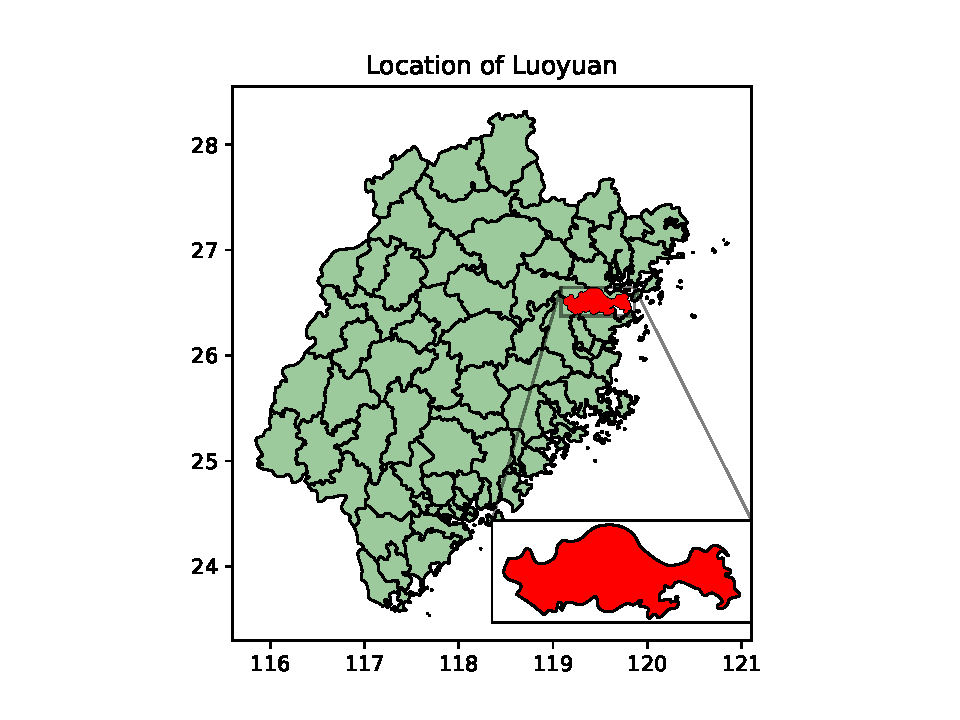
\includegraphics[width=0.6\textwidth]{./src/luoyuan.pdf}
\caption{研究区域}
\end{figure}
\subsubsection{栅格数据的几何校正}
对于MODIS栅格数据需要进行几何校正, 将栅格数据的位置信息重投影到WGS84坐标系下. 具体的过程是先建立一个虚拟数据集(GDAL Virtual Format, VRT)\cite{gdal}
将原有波段的数据包装成另一个数据集(GeoDataset), 并利用该数据集将原有数据校正到输出的数据集中\footnote{该表述参考了乐松山老师的课程Python与空间信息处理的PPT.}.
由于MODIS L1B 1km数据中的Metadata已经包括了地面控制点(GCP)的信息, 而根据GDAL的文档\cite{gdal}, \verb|gdal.Translate()|函数中的参数\verb|nogcp=False|, 所以应当不需要重新加入GCP, GDAL能够从输入数据中自行获取.
具体代码见\ref{geom_corr}. 

将几何校正后的其中一幅影像导入QGIS, 并叠加实际的世界地图, 如图\ref{res_geom_corr}, 可以看到几何校正的结果是正确的.
\begin{figure}[h]
\centering
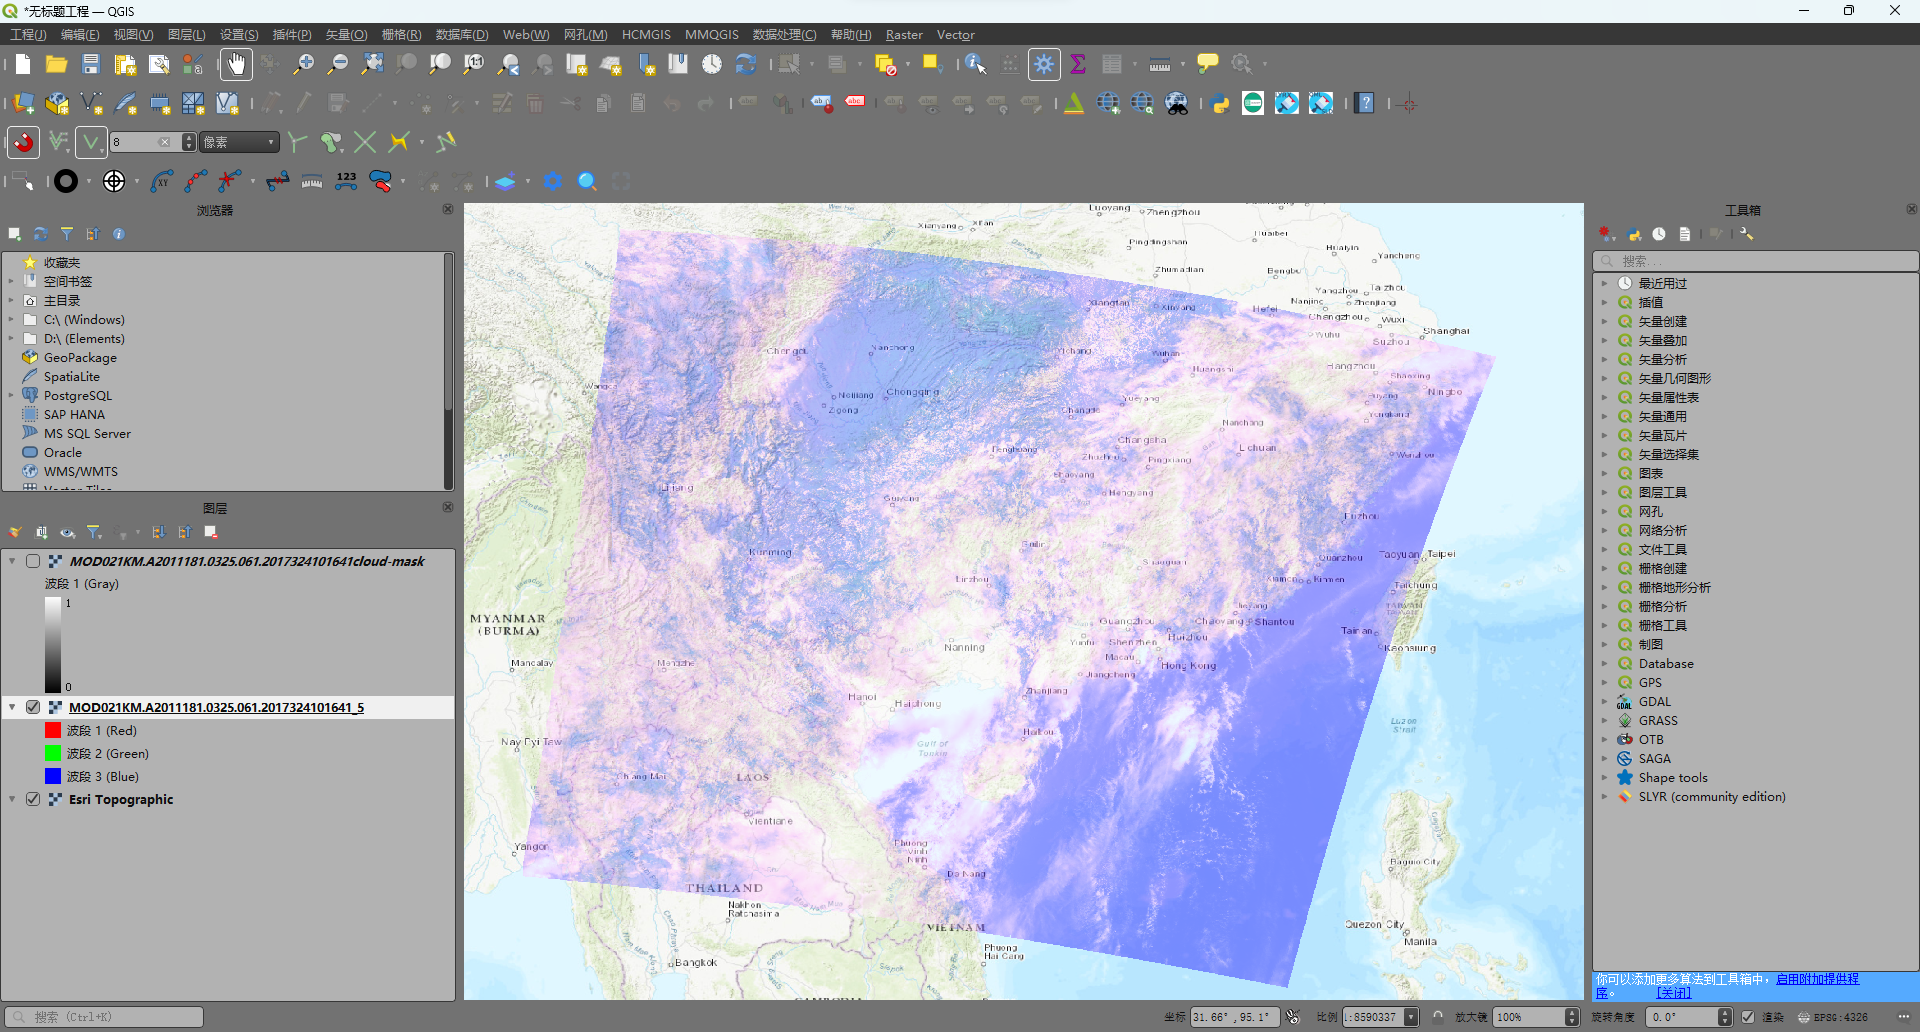
\includegraphics[width=0.6\textwidth]{./src/geom-corr.png}
\caption{几何校正的结果}\label{res_geom_corr}
\end{figure}
\subsubsection{栅格数据的辐射校正}\label{2-2-3}
辐射校正的过程是将遥感影像上的DN值转换为实际的辐亮度值$L$.
根据\textit{MODIS Level 1B Product User's Guide}可知, 辐亮度
\begin{align}
L=radiance\_scales \times \left( SI-radiance\_offsets\right)
\end{align}
因此需要在程序中对其进行计算.

同理, 由于所研究的对象是AOD, 因此还要进行表观反射率$\rho$的计算, 根据MODIS文档, 可知公式如下:
\begin{align}
\rho=\frac{reflectance\_scales \times (SI-reflectance\_offsets)}{\cos \Theta}
\end{align}
式中$\Theta$为太阳天顶角(入射角)\footnote{在\textit{MODIS Level 1B Product User's Guide}中表述为Solar incidence angel, 直译应为太阳入射角}

这一部分的代码见\ref{rad_corr}.

%对于气溶胶光学厚度反演, 需要获取MODIS 1KM表观反射率产品中的0.47$\mathrm{\mu}$m, 0.66$\mathrm{\mu}$m, 2.1$\mathrm{\mu}$m, 1.24$\mathrm{\mu}$m的波段, 这几个波段均在MODDIS的前7个波段中.

\subsubsection{栅格数据的云检测与去云}
云检测是遥感中必要的预处理步骤,
在本实验中根据\href{https://blog.csdn.net/ssshyeong/article/details/125947734}{\color{blue}链接}所引用的方法进行所用遥感影像的云检测. 
该方法提出了\textbf{CI}指数区分云和其它陆地物质, 由于MODIS具有多光谱数据, 该指数的表达为\cite{ZhaiZhang-707}
\begin{align}
\mathbf{CI}=\frac{\mathbf{B}_{NIR}+2\times \mathbf{B}_{SWIR-1}}{\mathbf{B}_B+\mathbf{B}_G+\mathbf{B}_R}
\end{align}
计算\textbf{CI}后通过下式监测云层
\begin{align}
\left|\mathbf{CI}-1\right|<T
\end{align}
其中$T$可以取$\{0.1,1,10,100\}$等值.

选取一张经过云检测的影像, 导入QGIS中, 如图\ref{cloud-test}, 图中黑色部分是检测出的云. 
\begin{figure}[h]\centering
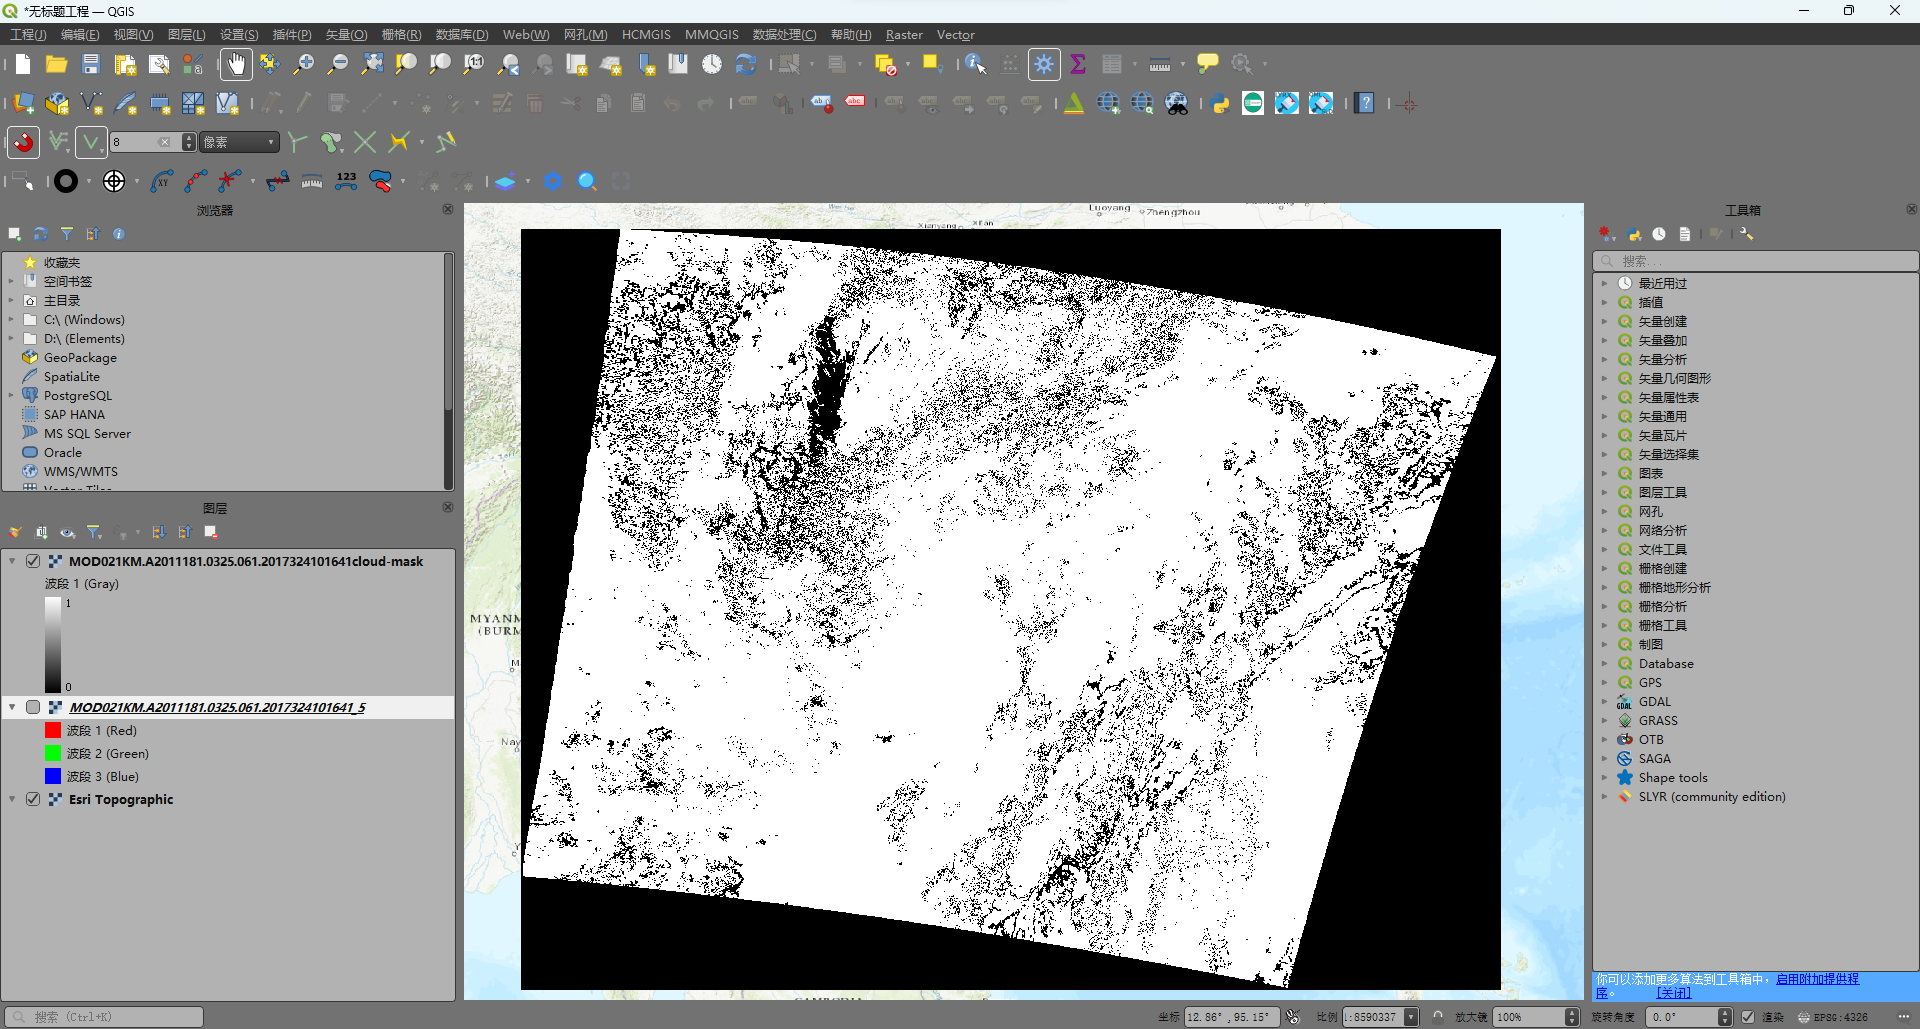
\includegraphics[width=0.8\textwidth]{./src/cloud-test.png}\caption{云检测}\label{cloud-test}
\end{figure}

云检测与去云的代码见\ref{cloud_test}.

\section{方法}
%\subsection{气溶胶光学厚度反演法}
\subsection{实验流程}
大气顶部反射率$\rho_{\mathrm{TOA}}$与气溶胶光学厚度有较为复杂的函数关系\cite{KaufmanTanri-708, 孙林于会泳-709}, 
本实验在实际计算中通过使用6S模型构建AOD与观测几何, 表观反射率和像元上的辐亮度之间的查找表, 并通过支持向量机回归(Support Vector Machine, SVM)分析AOD与输入参数之间的关系\footnote{实际上使用SVM的原因是我没有理解查找表的原理, 因此决定将其理解为回归, 最初使用的是线性回归, 但是个人认为因为大气传输模型的复杂性, 多元线性回归不能很好地拟合这个关系, 又想到课程中介绍的机器学习方法, 因此选择采用SVM回归.\label{process}}. 

\subsection{大气校正}
\subsubsection{6S模型}\label{6s}
6S模型是目前较为完善的大气辐射校正模型之一, 它是一个开源的模型, 由Fortran语言编写. 本人下载了6S\_V2.1的源码, 但是由于它是在Linux平台上构建的, Windows系统上缺少编译它的工具, 在Windows上进行配置较为复杂导致本人并没有成功编译它的程序. 
作为替代, 本实验使用了Python库\verb|Py6S|\cite{581987,WILSON2013166}对查找表进行构建. 

由于所研究的区域为福建省福州市罗源县, 该地区位于沿海, 且为城市区域,
时间为DOY181, 因此设置\verb|Py6S|的大气环境为中纬度夏季, 气溶胶参数为城市.

\subsubsection{查找表构建}
构建查找表需要设置观测几何参数等信息. 实验中根据\cite{陶金花李小英-705}
% 加一个参考文献引用
设置太阳天顶角为0$^\circ$,6$^\circ$,12$^\circ$,24$^\circ$, 35.2$^\circ$,48$^\circ$,54$^\circ$,60$^\circ$,66$^\circ$. 12个观测天顶角设置为0$^\circ$~66$^\circ$, 取12个相对方位角从0$^\circ$~180$^\circ$. 设置6个波长550nm处的大气气溶胶光学厚度值, 分别为0,0.25,0.5,1.0,1.5,1.95. 波段的中心波长取0.47$\mu$m,0.66$\mu$m,2.1$\mu$m.

通过\verb|Py6S|库运行之后可以得到查找表.

\subsubsection{暗像元法}
由\ref{2-2-3}中的描述, 我们已经计算过了表观反射率$\rho$的值, 并将其存储.

暗像元法的思想是由于地面辐射能量在2.1$\mu$m通道受大气气溶胶影响较小, 
因此近似认为该通道的地表反射率等于卫星接收到的表观反射率, 而0.47$\mu$m和0.66$\mu$m波段的地表反射率$R$与2.1$\mu$m处的表观反照率$\rho$存在以下关系\cite{李刚-706}:
\begin{align}
R_{0.47\mu\mathrm{m}}=\frac{1}{4}\rho_{2.1\mu\mathrm{m}}\\
R_{0.66\mu\mathrm{m}}=\frac{1}{2}\rho_{2.1\mu\mathrm{m}}.
\end{align}
但目前的问题是, 在使用\verb|Py6S|时, 发现无论如何设置大气模型, 只要不对模型中的``\textit{groud\_reflectance}''设置值, 则该项就为0, 这导致了回归时模型的地表反射率一项实际上没有起到作用. 

\subsection{SVM回归}
如注\ref{process}中所提到的, 本人没有理解查找表的用途, 因此所做的是根据本人的理解对查找表的值进行回归. 

SVM不仅支持线性和非线性分类, 同时它还支持线性和非线性回归\cite{Geron-710,Zhang-711}. 在本实验中, 采用了RBF(Radial Basis Function, 径向基核函数)核函数, 通常也被称为Gauss核函数. 它的表示如下\cite{Zhang-711}:
\begin{align}
K(\mathbf{x},\mathbf{x'})=\exp \left(\frac{-||\mathbf{x}-\mathbf{x'}||^2}{2\sigma^2}\right)
\end{align}
设置超参数$C$=\verb|10|, $\varepsilon$\verb|=0.1|. $C$为正则化参数, 而$\varepsilon$则表示在$\varepsilon$的范围内, 损失函数不会对其做出惩罚\cite{scikit-learn,Geron-710,Zhang-711}. 
(在附录所写的代码中还写了\verb|degree=2|, 但后来查找\verb|sklearn.svm|的文档后发现\verb|degree|在核函数不是\verb|poly|时都会被忽略).

计算得到拟合的得分为0.994, 按照\verb|sklearn.svm.SVR|的文档, \verb|score()|返回判定系数$R^2$(	
Return the coefficient of determination of the prediction), 如图\ref{score}. 由于设计实验时的失误, 进行SVM回归时没有划分训练集和验证集. 作为对比, 线性回归的score为0.74左右.
\begin{figure}[h]\centering
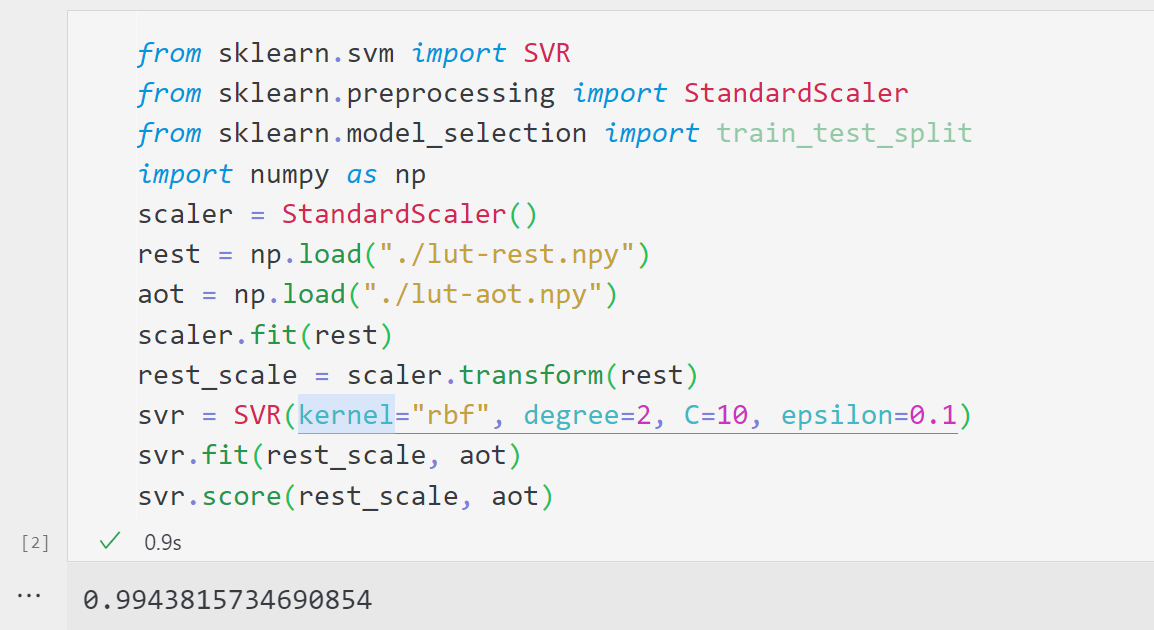
\includegraphics[width=.7\textwidth]{./src/score.png}
\caption{SVM回归的得分}\label{score}
\end{figure}

在进行SVM回归时要注意将输入数据进行归一化, 否则结果将出现问题. 在没有进行归一化的情况下$R^2$的数值会大幅减低, 效果甚至不如线性回归. 而在对实际数据进行AOD的预测时, 若忘记归一化, 则导致后果如图\ref{wrong}.
\begin{figure}[h]\centering
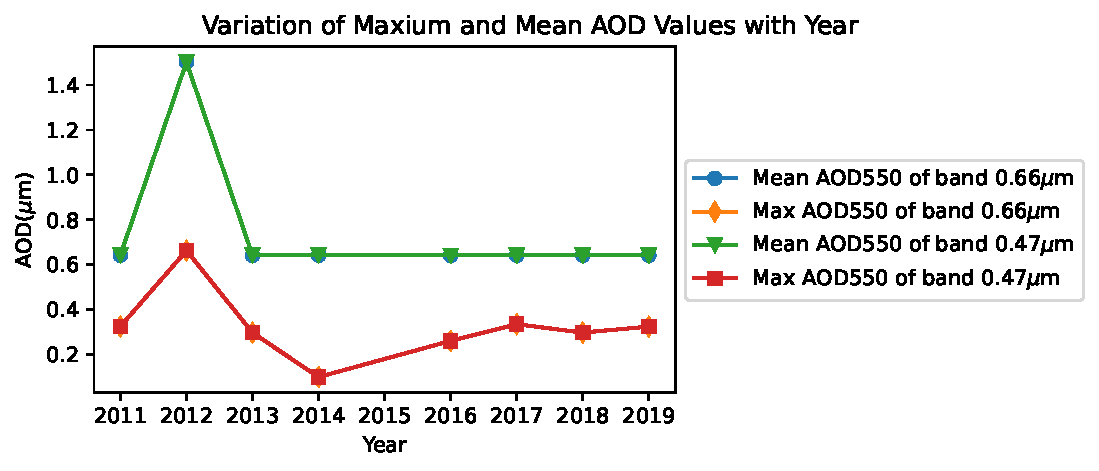
\includegraphics[width=0.6\textwidth]{./src/stat-wrong.pdf}
\caption{忘记归一化之后进行处理得到的AOD}\label{wrong}
\end{figure}

\subsection{根据DEM的高程校正AOD}
校正公式为
\begin{align}
\tau_Z=0.00877\times 0.55^{-4.05}\left(1-\exp\left(\frac{-Z}{8.5}\right)\right)+\tau_0
\end{align}
式中$\tau_Z$为经过海拔校正的AOD, $\tau_0$为根据查找表计算的, 即未经过海拔校正的AOD, $Z$为海拔, 单位为km.
\section{结果与讨论}
\subsection{结果}
通过对罗源县2011-2019年6月30日的气溶胶光学厚度的平均值和最大值进行可视化, 结果如图\ref{mean-max-aod}.
\begin{figure}[h]\centering
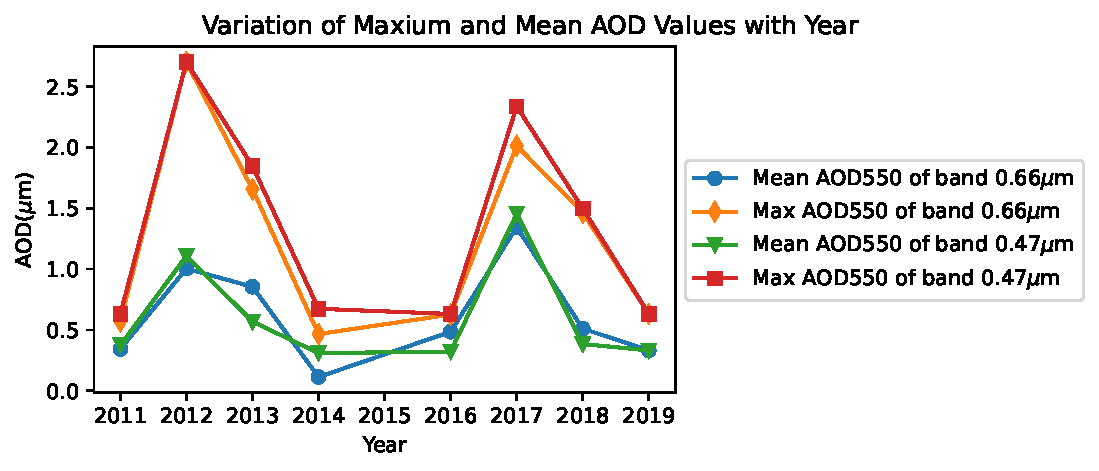
\includegraphics[width=.7\textwidth]{./src/stat.pdf}
\caption{各年度6月30日AOD平均值与最大值}\label{mean-max-aod}
\end{figure}
本实验所计算的2011-2019年6月30日罗源县气溶胶光学厚度值分布如图\ref*{res}.
\begin{figure}[!htbp]
\centering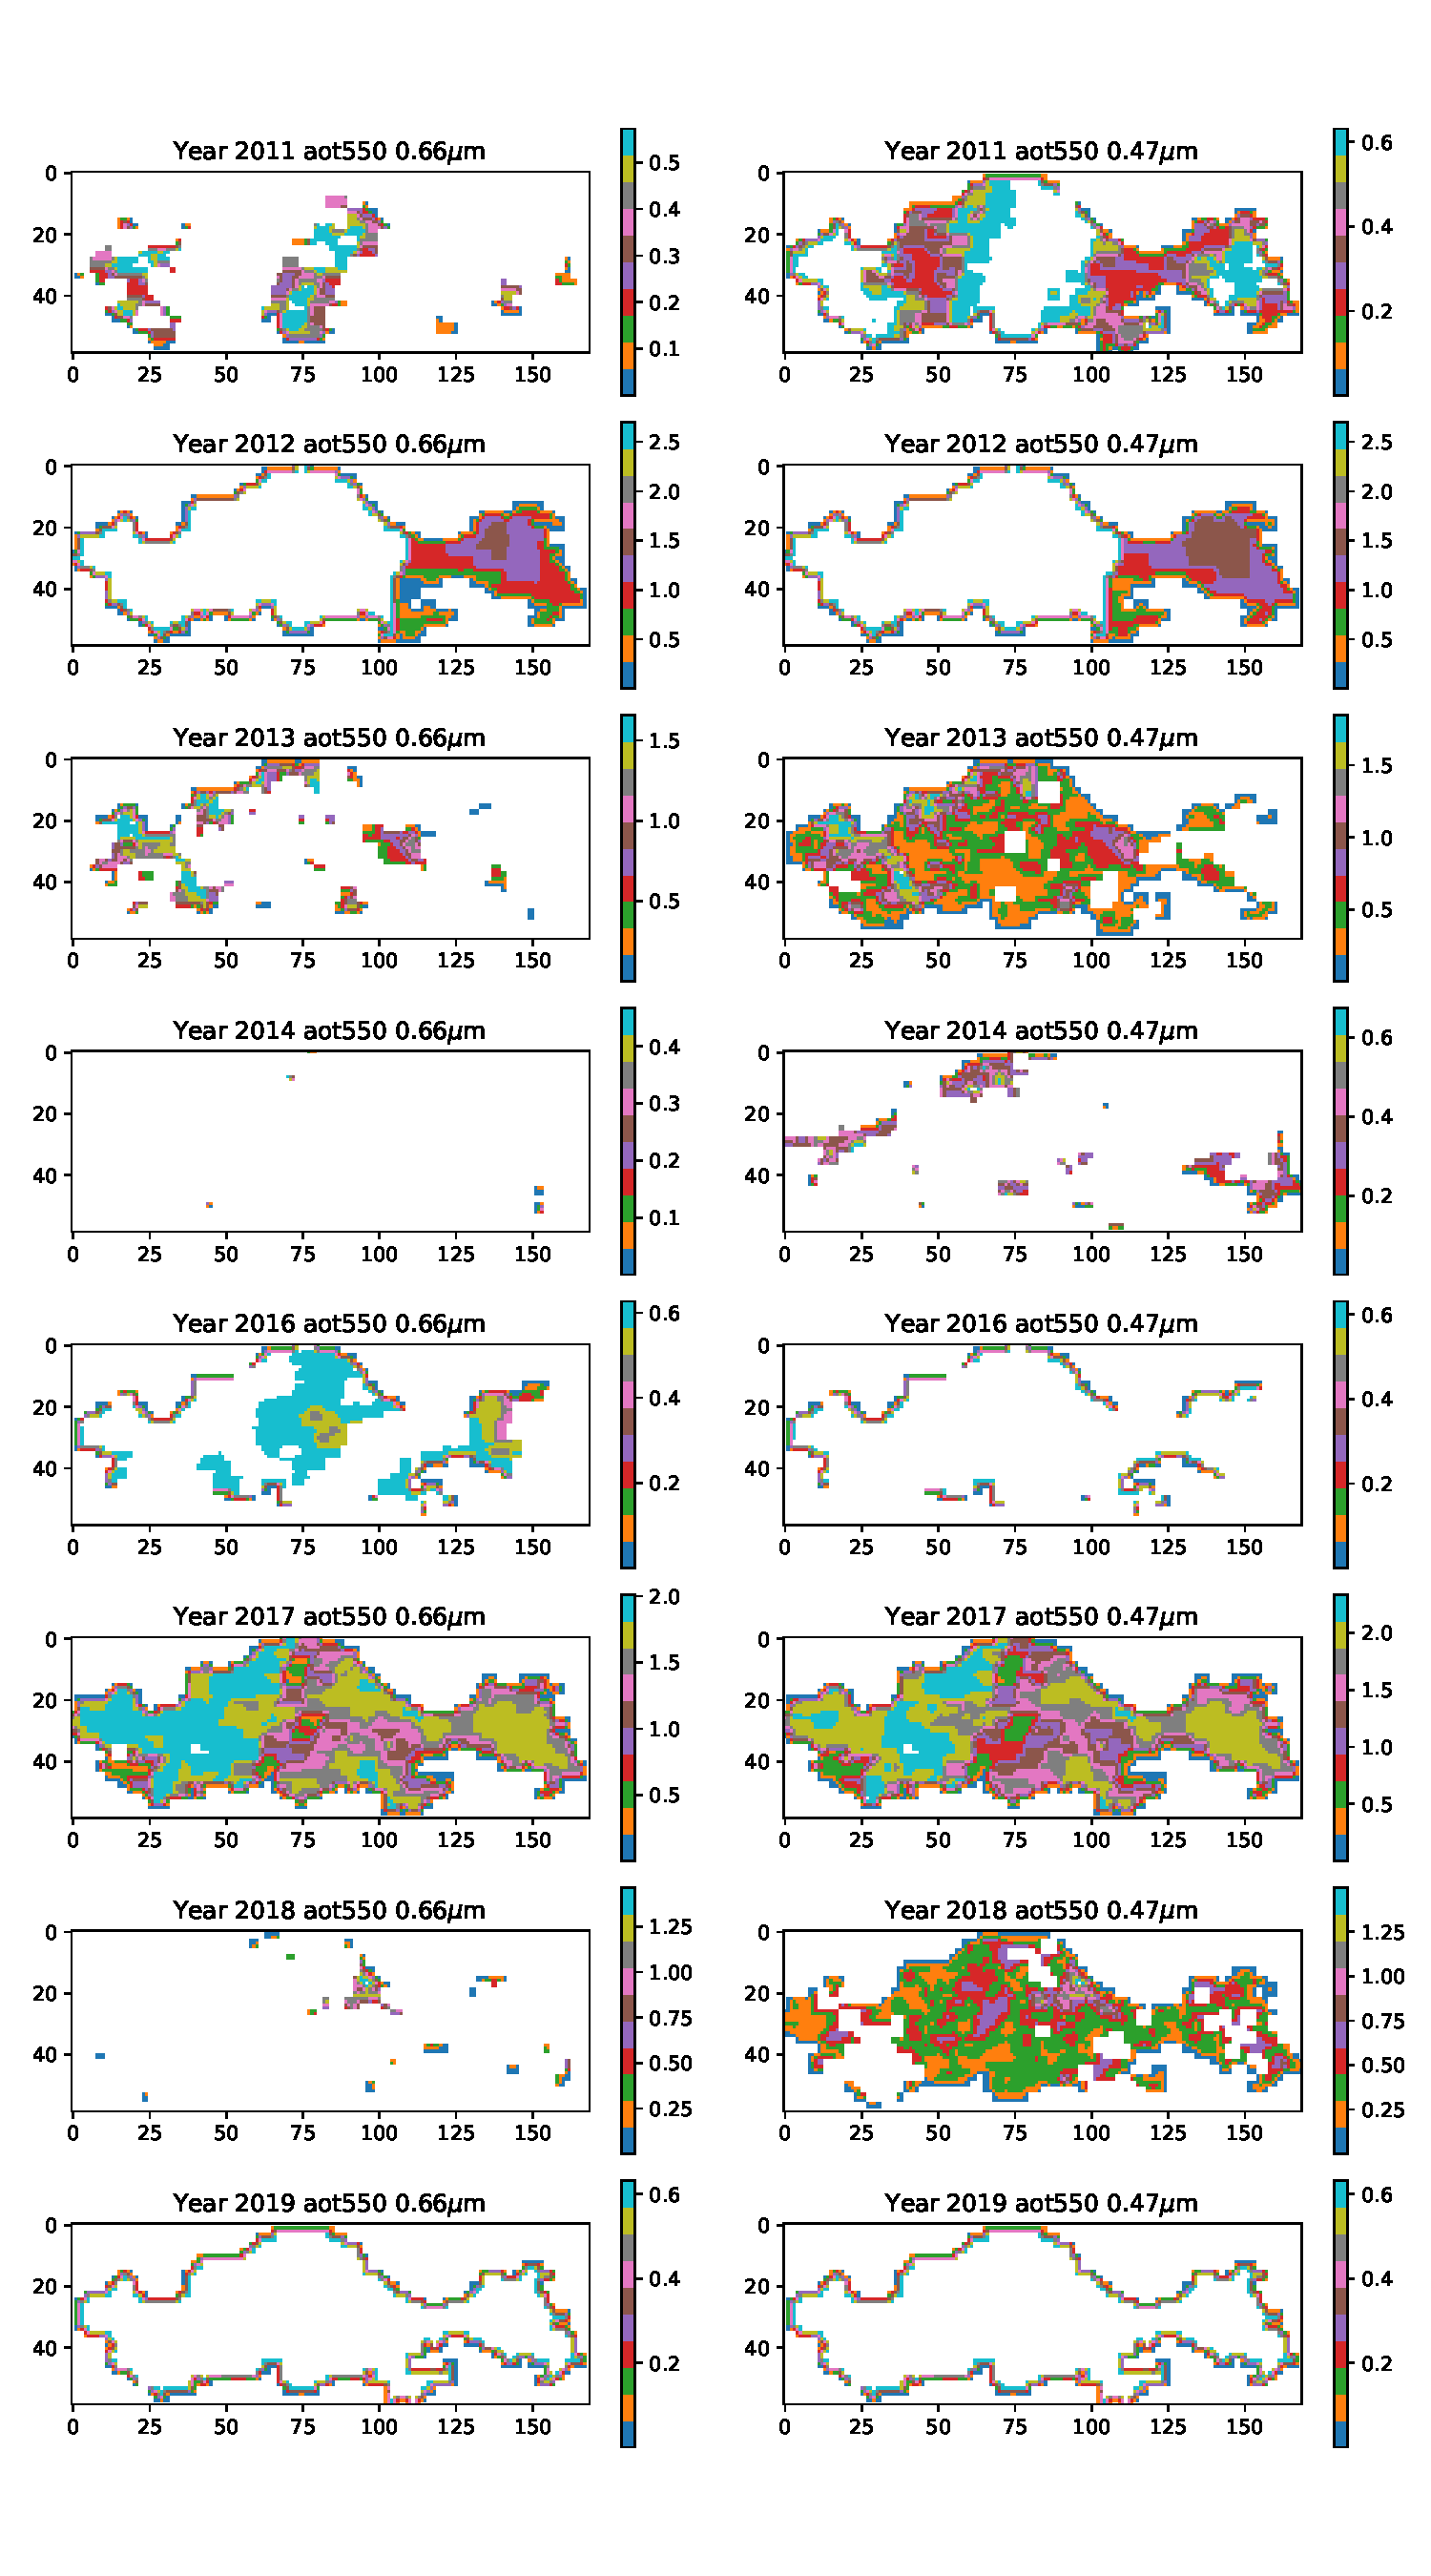
\includegraphics[width=0.65\textwidth]{./src/res2.pdf}
\caption{各年度6月30日罗源县AOD分布}\label{res}. 
\end{figure}
可列出各年度6月30日罗源县AOD值的平均值和最大值如表
\begin{table}
\begin{center}\caption{2011-2019年罗源县AOD平均值和最大值}\label{table-mean-max}
\begin{tabular}{c|cccc}
\Xhline{1.5pt}
 \multirow{2}*{年份} & \multicolumn{2}{c}{0.47$\mu$m波段} & \multicolumn{2}{c}{0.66$\mu$m波段} \\
 \cmidrule(lr){2-3}\cmidrule(lr){4-5}
 %\cline{2-3} \cline{4-5}
 ~ & 平均值 & 最大值 & 平均值 & 最大值 \\
\Xhline{1pt}
 2011 & 0.34347314 & 0.5720427 & 0.37455916 & 0.6309889\\
 2012 & 1.0044318 & 2.702205 & 1.1086358 & 2.702205 \\
 2013 & 0.85470253 & 1.6571355 & 0.56879723 & 1.8472286\\
 2014 & 0.11298013 & 0.46662354 & 0.3092775 & 0.67417115\\
 2016 & 0.4850499 & 0.62692034 & 0.32288575 & 0.6311006\\
 2017 & 1.345311 & 2.0139356 & 1.4545723 & 2.3368564\\
 2018 & 0.5108329 & 1.4644104 & 0.38467848 & 1.4981769\\
 2019 & 0.33165756 & 0.6316235 & 0.33165756 & 0.6316235\\
\Xhline{1.5pt}
\end{tabular}
\end{center}
\end{table}
\subsection{讨论}
图\ref{res}中白色部分是罗源县以外的区域, 或者在当时被云覆盖的区域. 
从图\ref{mean-max-aod}中可以看出, 在2012年的AOD值出现了异常增高的情况.
排查后没有发现原因, 因此猜测可能是数据预处理或计算时出现的错误.

整体而言, 在罗源闽光钢铁厂建立以后, 即以2015年为界, 罗源县的气溶胶光学厚度的平均值并没有明显上升趋势, 而在2017年以后AOD值甚至出现了下降的情况.
这一情况的原因很可能为所选取的遥感影像数据数量较少, 不足以形成统计规律. 同时由于环境政策和2015年中央经济工作部署中的``去产能'', ``去库存'', ``去杠杆'', ``降成本'', ``补短板''五大任务的推动, 导致大型钢铁企业的产能下降和环保投入提升, 所产生的污染也有所下降.

\section{结论}
本实验使用MODIS L1B 1km数据, 通过6S大气模型构建查找表,
对气溶胶光学厚度与观测几何, 表观反射率以及像元辐亮度进行SVM回归, 
从而对福州市罗源县2011-2019年6月30日气溶胶光学厚度进行反演, 分析自2014年罗源闽光钢铁厂建立以来对罗源县气溶胶光学厚度的影响. 
经过数据处理与分析, 根据所选用的数据, 没有发现以2015年为界, 罗源县的气溶胶光学厚度有显著性增加, 因此不能认为该钢铁企业的建立导致当地空气质量下降. 

由于本实验所选取的数据较少, 对于研究内容的代表性不足, 后续改进方向可以是增加所获取的遥感影像数量; 
此外本实验所选取的部分遥感影像云量过多, 导致部分区域能够用于反演AOD的数据量较小, 在数据量提升之后需要对云量过多的图像加以剔除;
本实验在对气溶胶进行SVM回归时没有划分训练集和验证集, 因此回归的结果很可能存在过拟合的现象, 其中2019年反演得到的气溶胶光学厚度值全为同一个值, 因此在本实验可视化的过程中均将其剔除.

\bibliographystyle{apalike}
\bibliography{./src/ref.bib}

\part*{附录}\label{appendices}
\addcontentsline{toc}{part}{附录}
附录部分主要包括以上进行遥感数据处理的主要Python代码.
可运行的ipynb文件可通过本人GitHub主页\textcolor{blue}{\href{https://yhw605.github.io}{https://yhw605.github.io}}获取(还需要再进行整理, 所以可能暂时没有放上去, 未整理完成的Jupyter Notebook文件可联系\href{mailto:hanwen_yan@outlook.com}{\textcolor{blue}{本人邮箱})}. 但是由于数据过于庞大, 因此所有MODIS L1B 1km数据的文件以及数据处理后所生成的新文件不会在链接中提供, 而仅提供数据名称.
\begin{appendices}

\section{读取数据}
\subsection{读取GDB数据}\label{readgdb}
\begin{lstlisting}[frame=single, basicstyle={\ttfamily}, language = Python, caption={读取GDB并输出为shp}, label = {out}]

import geopandas as gpd
from osgeo import ogr
import matplotlib.pyplot as plt
import os
from sklearn.ensemble import RandomForestClassifier

# 读取 Geodatabase 格式数据
fjgdb_file = "./fjgdb/福建省地图示意图版.gdb/"
fjgdb = ogr.Open(fjgdb_file)

# 获取各个图层的名称
lyr_size = fjgdb.GetLayerCount()
for i in range(lyr_size):
    lyr = fjgdb.GetLayerByIndex(i)
    name = lyr.GetName()
    # print(name)
    
for i in range(lyr_size):
    lyr = fjgdb.GetLayer(i)
    # print(lyr)
    driver = ogr.GetDriverByName("ESRI Shapefile")
    out_ds = driver.CreateDataSource("./shp-data/" + lyr.GetName() + ".shp")
    out_lyr = out_ds.CreateLayer(lyr.GetName(), 
                                 lyr.GetSpatialRef(), lyr.GetGeomType())
    lyr_defn = lyr.GetLayerDefn()
    feature = lyr.GetNextFeature()
    while feature:
        out_lyr.CreateFeature(feature)
        
        feature = lyr.GetNextFeature()
    
    out_ds.Destroy()

map_df = gpd.read_file("./shp-data/县级行政区.shp")
map_df = map_df.to_crs(epsg=4326)
luoyuan = map_df[map_df["FID"] == 54]
fig, ax = plt.subplots()
map_df.plot(edgecolor='k', facecolor='#9CCA9C', alpha=1, ax=ax)
luoyuan.plot(color='r', ax=ax)
sub_map = ax.inset_axes([0.5, 0.0, 0.5, 0.25], transform=ax.transAxes)
sub_map.grid(False)
sub_map.tick_params(which='both',
                     labelleft=False, left=False,
                     bottom=False, labelbottom=False)
insert_map = luoyuan.plot(color='r', edgecolor='k', ax=sub_map)
ax.indicate_inset_zoom(sub_map, edgecolor='k', lw=1.2)
plt.title("Location of Luoyuan")
plt.savefig("./visualization/luoyuan.pdf")

luoyuan.to_file("./shp-data/luoyuan.shp",
                 driver="ESRI Shapefile", encoding="utf-8")

\end{lstlisting}
\subsection{读取栅格数据}
由于后续所有操作都需要读取栅格数据, 因此不在此处展示. 读取栅格数据主要使用的是Python库\verb|gdal|和\verb|rasterio|. 
\section{数据预处理}
\subsection{几何校正}\label{geom_corr}
本部分代码主要参考了\href{https://blog.csdn.net/kymgoal/article/details/112150360}{https://blog.csdn.net/kymgoal/article/details/112150360}中的代码.
\begin{lstlisting}[frame=single, language=Python,  basicstyle={\ttfamily}, caption={几何校正}, label=codegeom_corr]
import os
from osgeo import gdal


def swath_georeference(in_file, geo_file,
                      target_dataset_name, out_file,
                      out_geo_range, x_res_out, y_res_out):
    dataset = gdal.Open(in_file)
    subdatasets = dataset.GetSubDatasets()
    dataset_pos = 0
    target_pos = 0#-1
    for subdataset in subdatasets:
        subdataset_name = subdataset[0]
        if subdataset_name.endswith(target_dataset_name):
            target_pos = dataset_pos
        dataset_pos += 1
        
        if target_pos != -1:
            target_dataset = dataset.GetSubDatasets()[target_pos][0]
            vrt_file = os.path.splitext(in_file)[0] + '.vrt'
            vrt_out = gdal.Translate(vrt_file, target_dataset,
                                     format='vrt', unscale='true')
            georeferenced_data = gdal.Warp(out_file\
                             +"_"+str(target_pos+1)+".tif",
                              vrt_out, multithread=True,
                              outputBounds=out_geo_range,
                              format='GTiff', geoloc=True,
                              dstSRS="EPSG:4326",
                              xRes=x_res_out,
                              yRes=y_res_out,
                              dstNodata=0.0,
                              outputType=gdal.GDT_Float32)
            target_pos += 1
            print(
                 'The georeference of {} is complete.'.format(in_file))
            os.remove(vrt_file)
        else:
            print('{} has no the target dataset.'.format(in_file))


def main():
    file_prefix = '.hdf'
    input_directory = './hdfs/'
    output_directory = './hdf-output/'
    if not os.path.exists(output_directory):
        os.mkdir(output_directory)
    file_list = os.listdir(input_directory)
    for file_i in file_list:
        if file_i.endswith(file_prefix):
            file_name = input_directory + file_i
            out_file = output_directory\
             + os.path.splitext(file_i)[0]# + '_geo.tiff'
            dataset_name = 'Image_Optical_Depth_Land_And_Ocean'
            geo_range = None  # [90.0, 55.0, 120.0, 25.0]
            x_res = 0.01
            y_res = 0.01
            swath_georeference(file_name, file_name,
                               dataset_name, out_file, geo_range,
                               x_res, y_res)


if __name__ == '__main__':
    main()


\end{lstlisting}
\subsection{辐射校正}\label{rad_corr}
%\subsection{辐射校正}
\begin{lstlisting}[frame=single, language=Python,  basicstyle={\ttfamily}, caption={辐射校正}, label=coderad_corr]
from osgeo import gdal, osr, gdalconst
from osgeo import ogr
import geopandas as gpd
import numpy as np
import matplotlib.pyplot as plt
import re
import copy
import os
import cv2

folder_path = "./hdf-output/"
for filename in os.listdir(folder_path):
    #print(filename[-6:-4])
    if filename[-6:-4] == "_5" or filename[-6:-4] == "_8": 
        # MODDIS前7个波段的数据
        print(filename)
        hdf_name = "./hdfs/" + filename[:-6] + ".hdf"
        hdf_data = gdal.Open(hdf_name)
        solar_zenith_data = gdal.Open(hdf_data.GetSubDatasets()[14][0])
        # 太阳天顶角 它的角度范围是0-18000, 所以要除200 并化到0-pi
        zenith = np.deg2rad(
            solar_zenith_data.GetRasterBand(1).ReadAsArray() / 200)

        data = gdal.Open(folder_path + filename)
        rad_off = data.GetMetadataItem("radiance_offsets")
        rad_off = np.array(
                rad_off.replace(' ', '').split(","), dtype=np.float64)
        rad_scales = data.GetMetadataItem("radiance_scales")
        rad_scales = np.array(
                rad_scales.replace(' ', '').split(","), dtype=np.float64)
        ref_off = data.GetMetadataItem("reflectance_offsets")
        ref_off = np.array(
            ref_off.replace(' ', '').split(","), dtype=np.float64)
        ref_scale = data.GetMetadataItem("reflectance_scales")
        ref_scale = np.array(
            ref_scale.replace(' ', '').split(","), dtype=np.float64)
        band_size = data.RasterCount
        driver = gdal.GetDriverByName("GTiff")
        out_ds = driver.Create("./rad-corr/" + filename, 
                                data.RasterXSize, data.RasterYSize,
                                band_size*2, gdal.GDT_Int64)
        for i in range(1,band_size+1):
            band = data.GetRasterBand(i).ReadAsArray()
            corr_band = (band - rad_off[i-1]) * rad_scales[i-1]
            # 辐射
            out_band = out_ds.GetRasterBand(i)
            # 反射
            ref_band = out_ds.GetRasterBand(i + band_size)
            # 重采样太阳天顶角的数据
            z = cv2.resize(zenith, dsize=corr_band.shape,
                            interpolation=cv2.INTER_LINEAR)
            # 计算反射率
            ref = ref_scale[i-1] * (band - ref_scale[i-1]) / np.cos(z).T
            # 将反射率映射到扩大1000背, 因为类型是Int32
            ref = ref * 1000
            out_band.WriteArray(corr_band)
            ref_band.WriteArray(ref)
            print(ref.max(), ref.min(), ref.mean())
            ref2 = out_ds.GetRasterBand(i + band_size).ReadAsArray()
            print(ref2.max(), ref2.min(), ref2.mean())
            pass
        out_ds.SetProjection(data.GetProjection())
        out_ds.SetGeoTransform(data.GetGeoTransform())
        out_ds.FlushCache()
        out_ds = None
        pass
\end{lstlisting}
\subsection{云检测与去云}\label{cloud_test}
\begin{lstlisting}[frame=single, language=Python, basicstyle={\ttfamily}, caption={云检测}, label=codecloud]
from osgeo import gdal, ogr, osr
from sklearn.ensemble import RandomForestClassifier
import cv2
import os
import matplotlib.pyplot as plt
import numpy as np

folder_path = "./rad-corr/"
flist = os.listdir(folder_path)
for i in range(0, len(flist), 2):
    print(flist[i])
    if flist[i][-4:] != ".tif":
        continue
    half = gdal.Open(folder_path + flist[i+1]) # 500m分辨率波段
    quater = gdal.Open(folder_path + flist[i]) # 250m
    red_band = quater.GetRasterBand(1).ReadAsArray() # 红光波段
    nir_band = quater.GetRasterBand(2).ReadAsArray()
    green_band = half.GetRasterBand(2).ReadAsArray()
    blue_band = half.GetRasterBand(1).ReadAsArray()
    swir_band = half.GetRasterBand(3).ReadAsArray() # 短波红外, 该band的SNR较低

    x,y=nir_band.shape
    swir_band = cv2.resize(swir_band, dsize=(y,x),
                            interpolation=cv2.INTER_LINEAR)
    blue_band = cv2.resize(blue_band, dsize=(y,x),
                            interpolation=cv2.INTER_LINEAR)
    green_band = cv2.resize(green_band, dsize=(y,x),
                            interpolation=cv2.INTER_LINEAR)
    
    ci = (nir_band + 2 * swir_band) / (red_band + green_band + blue_band)
    ci = np.nan_to_num(ci, 1)
    # https://blog.csdn.net/ssshyeong/article/details/125947734
    # 云检测 
    ci[np.fabs(ci - 1) < 1] = 1
    ci[np.fabs(ci - 1) >= 1] = 0
    out_ds = gdal.GetDriverByName("GTiff").Create(
        "./cloud_mask/" + flist[i][:-6]+"cloud-mask.tif", 
        quater.RasterXSize, quater.RasterYSize, 1, gdal.GDT_Int64)
    
    out_ds.WriteArray(ci)
    out_ds.SetGeoTransform(quater.GetGeoTransform())
    out_ds.SetProjection(quater.GetProjection())
    out_ds.FlushCache()
    out_ds = None
\end{lstlisting}
\begin{lstlisting}[frame=single, language=Python, basicstyle={\ttfamily}, caption={去云}, label=coderemove-cloud]
# 去云
from osgeo import gdal, ogr, osr
# from sklearn.ensemble import RandomForestClassifier
import cv2
import os
# import matplotlib.pyplot as plt
import numpy as np

folder_path = "./rad-corr/"
cloud_path = "./cloud_mask/"
out_path = "./cloud-clip/"
cloud_list = os.listdir(cloud_path)
flist = os.listdir(folder_path)
# i = 0
for i in range(0, len(flist), 2):
    if flist[i][-4:] != ".tif":
        continue
    quater = gdal.Open(folder_path + flist[i]) # 250m  
    half = gdal.Open(folder_path + flist[i+1]) # 500m
    cloud = gdal.Open(cloud_path + cloud_list[i % 2]) # 云掩膜
    cloud_band = cloud.GetRasterBand(1).ReadAsArray()
    out_ds = gdal.GetDriverByName("GTiff").Create(
        out_path + flist[i][:-4] + "cloud-clip22.tif", 
        quater.RasterXSize, quater.RasterYSize, (2+5)*2, gdal.GDT_Int64)
    # 读取每一个波段的数据
    band_list = []
    band_list.append(quater.GetRasterBand(1).ReadAsArray())
    band_list.append(quater.GetRasterBand(2).ReadAsArray())
    band_list.append(quater.GetRasterBand(3).ReadAsArray())
    band_list.append(quater.GetRasterBand(4).ReadAsArray())
    band_list.append(half.GetRasterBand(1).ReadAsArray())
    band_list.append(half.GetRasterBand(2).ReadAsArray())
    band_list.append(half.GetRasterBand(3).ReadAsArray())
    band_list.append(half.GetRasterBand(4).ReadAsArray())
    band_list.append(half.GetRasterBand(5).ReadAsArray())
    band_list.append(half.GetRasterBand(6).ReadAsArray())
    band_list.append(half.GetRasterBand(7).ReadAsArray())
    band_list.append(half.GetRasterBand(8).ReadAsArray())
    band_list.append(half.GetRasterBand(9).ReadAsArray())
    band_list.append(half.GetRasterBand(10).ReadAsArray())
    j = 0
    for band in band_list:
        #out_band = out_ds.GetRasterBand(j+1).ReadAsArray()
        out_band = band
        x, y = band.shape
        resize_cloud = cv2.resize(cloud_band+0.0001, dsize=(y,x), 
                                  interpolation=cv2.INTER_LINEAR)
        out_band[resize_cloud == 0.0] = 255
        # out_band[cloud_band != 1.0] = band
        #print(out_band.max(), out_band.min(), out_band.mean())
        out2 = out_ds.GetRasterBand(j+1)
        out2.WriteArray(out_band)
        out3 = out_ds.GetRasterBand(j+1)
        kkkkk = out3.ReadAsArray()
        print(kkkkk.mean())
        j+=1
        #for k in range(row):
        #    for m in range(col):
        #        if cloud_band[k][m] == 1.0:
        #            out_band[k][m] = 65535.0
        #        else:
        #            out_band[k][m] = band[k][m]
        #pass
    out_ds.SetProjection(quater.GetProjection())
    out_ds.SetGeoTransform(quater.GetGeoTransform())
    out_ds.FlushCache()
    out_ds = None
    print(out_path + flist[i][:-4] + "cloud-clip.tif" + " complete clip!")
    pass

\end{lstlisting}
\section{模型构建与计算}\subsection{构建查找表}\label{lut}
\begin{lstlisting}[frame=single, language=Python, basicstyle={\ttfamily}, caption={构建查找表}]
from Py6S import *
from osgeo import gdal, ogr, osr
import numpy as np
import cv2

sza_range = np.array([0,6,12,24,35.2,48,54,60])
saa_range = np.linspace(0, 72, 6)
vza_range = np.linspace(0,180, 12)
wvl_range = np.array([0.47,0.66,2.1]) * 1000
aot_range = np.array([0,0.25,0.5,1.,1.5,1.95])
res = []
i = 0
for sza in sza_range:
    for saa in saa_range:
        for vza in vza_range:
            for wvl in wvl_range:
                for aot in aot_range:
                    s = SixS()
                    s.atmos_profile = AtmosProfile.PredefinedType(
                        AtmosProfile.MidlatitudeSummer)
                    s.aero_profile = AeroProfile.Urban # 所研究的区域是城市
                    s.geometry.solar_a = saa
                    s.geometry.solar_z = sza
                    s.wavelength = Wavelength(wvl/1000)
                    s.aot550 = aot
                    s.geometry.view_a = vza
                    #s.ground_reflectance = GroundReflectance.HomogeneousLambertian([0,.1,.2])
                    #wavelengths, results = SixSHelpers.Wavelengths.run_modis(s, output_name="aot550")
                    s.run()
                    res.append([s.outputs.values])
                    print(len(res))
\end{lstlisting}
\subsection{SVM回归}
\subsubsection{训练数据}
\begin{lstlisting}[frame=single, language=Python, label=train, basicstyle={\ttfamily}, caption={训练数据}]
# 构造数据集
aot = []
rest = []
for val in res:
    aot.append(val[0]["aot550"])
    rest2 = np.array([val[0]["solar_a"],val[0]["solar_z"]-  
                      val[0]["view_z"], val[0]["view_a"],
                      val[0]["pixel_radiance"], 
                      val[0]["apparent_reflectance"], 
                      val[0]["background_reflectance"]])
    rest.append(rest2)
aot = np.array(aot)
rest = np.array(rest)

# 保存数据集
np.save("lut-aot.npy", aot)
np.save("lut-rest.npy", rest)

# 训练数据
from sklearn.svm import SVR
from sklearn.preprocessing import StandardScaler
from sklearn.model_selection import train_test_split
import numpy as np
scaler = StandardScaler()
rest = np.load("./lut-rest.npy")
aot = np.load("./lut-aot.npy")
scaler.fit(rest)
rest_scale = scaler.transform(rest)
svr = SVR(kernel="rbf", degree=2, C=10, epsilon=0.1)
svr.fit(rest_scale, aot)
svr.score(rest_scale, aot)
\end{lstlisting}
\subsubsection{计算AOD}
这个代码块在本人的计算机环境下运行一次要一小时.
\begin{lstlisting}[frame=single, language=Python, basicstyle={\ttfamily}, label=fit, caption={计算AOD}]
# 经过几何校正的数据, 它包含了没有被后续读取的太阳和传感器的角度信息
import os
hdf_path = "./hdf-output/" 
folder_path = "./cloud-clip/"

for fname in os.listdir(folder_path):
    if fname.startswith("M") == False or fname[-4:] != ".tif":
        continue
    elif fname.find("A2015") != -1 or fname.find("A2012182.0335") != -1:
        continue # 这两块数据有缺失
    solar_a = gdal.Open(
        hdf_path + fname[:-18] + "_18.tif")
    solar_a = solar_a.GetRasterBand(1).ReadAsArray() / 200
    solar_z = gdal.Open(
        hdf_path + fname[:-18] + "_19.tif")
    solar_z = solar_z.GetRasterBand(1).ReadAsArray() / 200
    view_a = gdal.Open(
        hdf_path + fname[:-18] + "_16.tif")
    view_a = view_a.GetRasterBand(1).ReadAsArray() / 200
    view_z = gdal.Open(
        hdf_path + fname[:-18] + "_17.tif")
    view_z = view_z.GetRasterBand(1).ReadAsArray() / 200
    band = gdal.Open(folder_path + fname)
    blue_band = band.GetRasterBand(3).ReadAsArray() # 0.47um
    red_band = band.GetRasterBand(1).ReadAsArray() # 0.66um
     # 0.47的表观反射率
    red_band_ref = band.GetRasterBand(8).ReadAsArray()/1000
    # 0.66的表观反射率
    blue_band_ref = band.GetRasterBand(10).ReadAsArray()/1000
    swir_band = band.GetRasterBand(7).ReadAsArray() # 2.1um
    swir_band_ref = band.GetRasterBand(14).ReadAsArray()/1000 # 2.1um
    # 重采样
    x, y = blue_band.shape
    view_a = cv2.resize(view_a+0.0001, dsize=(y,x), 
                        interpolation=cv2.INTER_LINEAR)
    solar_a = cv2.resize(solar_a+0.0001, dsize=(y,x), 
                         interpolation=cv2.INTER_LINEAR)
    view_z = cv2.resize(view_z+0.0001, dsize=(y,x), 
                        interpolation=cv2.INTER_LINEAR)
    solar_z = cv2.resize(solar_z+0.0001, dsize=(y,x), 
                         interpolation=cv2.INTER_LINEAR)
    red_aot = swir_band_ref.copy()
    blue_aot = swir_band_ref.copy()
    para1 = np.array([solar_a[red_aot < 0.26], 
                     solar_z[red_aot < 0.26] - view_z[red_aot < 0.26], 
                     view_a[red_aot < 0.26], 
                     red_band[red_aot < 0.26], 
                     red_band_ref[red_aot < 0.26], 
                     swir_band_ref[red_aot < 0.26]/4])
    para2 = np.array([solar_a[red_aot < 0.26], 
                     solar_z[red_aot < 0.26] - view_z[red_aot < 0.26], 
                     view_a[red_aot < 0.26], 
                     blue_band[red_aot < 0.26], 
                     blue_band_ref[red_aot < 0.26], 
                     swir_band_ref[red_aot < 0.26]/2])
    para1 = para1.T
    para2 = para2.T
    red_aot[swir_band_ref < 0.26] = svr.predict(
        scaler.transform(para1))
    print("Complete red aod.")
    red_aot[swir_band_ref >= 0.26] = np.nan
    red_aot[red_aot < 0] = np.nan
    blue_aot[swir_band_ref < 0.26] = svr.predict(
        scaler.transform(para2))
    print("Complete blue aod.")
    blue_aot[swir_band_ref >= 0.26] = np.nan
    blue_aot[blue_aot < 0] = np.nan
    red_aot.reshape(x,y)
    blue_aot.reshape(x,y)
    out_ds = gdal.GetDriverByName(
    		"GTiff").Create("./aot550/"+fname, 
             y,x,2,gdal.GDT_Float32)
    out_red = out_ds.GetRasterBand(1)
    out_red.WriteArray(red_aot)
    out_blue = out_ds.GetRasterBand(2)
    out_blue.WriteArray(blue_aot)
    out_ds.SetGeoTransform(band.GetGeoTransform())
    out_ds.SetProjection(band.GetProjection())
    print(fname + " extracts aot completed")
    out_ds.FlushCache()
    out_ds = None
\end{lstlisting}
\section{使用矢量数据掩膜提取研究区域}
主要是分为对AOD和观测集合参数提取区域两部分, 
两部分代码有多处相同, 因为编写程序时是在Jupyter Notebook中写的, 所以对程序的模块化没有加以考虑. 
对DEM的掩膜提取因为只有一张影像, 故直接在QGIS软件中操作. 
\begin{lstlisting}[frame=single, language=Python, basicstyle={\ttfamily}, label=mask, caption={对研究区域掩膜提取}]
# https://zhuanlan.zhihu.com/p/596897568
import rasterio
from rasterio.mask import mask
import fiona
import os

# 对AOD
folder_path = "./aot550/"
shp = fiona.open("./shp-data/luoyuan.shp", "r", encoding="utf-8")
geoms = [feature["geometry"] for feature in shp]
for fname in os.listdir(folder_path):
    if fname[-4:] != ".tif": #or fname.find("A2019") != -1:
        continue
    with rasterio.open(folder_path + fname) as src:
        out_img, out_trans = mask(src, geoms, crop=True)
        out_meta = src.meta.copy()
    out_meta.update({"driver": "GTiff",
                     "height": out_img.shape[1],
                     "width": out_img.shape[2],
                     "transform": out_trans})
    with rasterio.open("./clipped/"+fname[:-4]+"clipped.tif", 
                       "w", **out_meta) as dest:
        dest.write(out_img)
    print(fname + " clipped!")

# 对观测几何参数
folder_path = "./hdf-output/"
shp = fiona.open("./shp-data/luoyuan.shp", "r", encoding="utf-8")
geoms = [feature["geometry"] for feature in shp]
for fname in os.listdir(folder_path):
    if fname[-4:] != ".tif" or fname[-7:-4] not in [
        "_16","_17","_18","_19"] or fname.find(
            "A2015") != -1 or fname.find("A2012182.0335") != -1:
        #print(fname[-7:-4])
        continue
    with rasterio.open(folder_path + fname) as src:
        out_img, out_trans = mask(src, geoms, crop=True)
        out_meta = src.meta.copy()
    out_meta.update({"driver": "GTiff",
                     "height": out_img.shape[1],
                     "width": out_img.shape[2],
                     "transform": out_trans})
    with rasterio.open("./hdf-out-clip/"+fname[:-4]+"clipped.tif", 
                       "w", **out_meta) as dest:
        dest.write(out_img)
    print(fname + " clipped!")
\end{lstlisting}
\section{对AOD的高程纠正}
\begin{lstlisting}[frame=single, language=Python, basicstyle={\ttfamily}, label=ele-corr, caption={对AOD的高程纠正}]
# 对AOD做高程的纠正并输出各年份的统计信息
from osgeo import gdal
import cv2
import numpy as np
import os
import pandas as pd

stat = pd.DataFrame()
blue_arr_mean = []
red_arr_mean = []
blue_arr_max = []
red_arr_max = []

folder_path = "./clipped/"
ele_data = gdal.Open("./luoyuan-elevation-km.tif")
el = ele_data.GetRasterBand(1).ReadAsArray()
for fname in os.listdir(folder_path):
    if fname[-4:] != ".tif":
        continue
    data = gdal.Open(folder_path + fname, gdal.GA_ReadOnly)
    red_aot = data.GetRasterBand(1).ReadAsArray()
    blue_aot = data.GetRasterBand(2).ReadAsArray()
    x, y = el.shape
    red_aot = cv2.resize(red_aot, dsize=(y, x), 
                         interpolation=cv2.INTER_LINEAR)
    blue_aot = cv2.resize(blue_aot, dsize=(y, x), 
                         interpolation=cv2.INTER_LINEAR)
    red_aot2 = red_aot.copy()
    red_aot2[red_aot != 0] = 0.00877 * 0.55**-4.05 * \
        (1-np.exp(-el[red_aot != 0]/8.5)) \
            + red_aot[red_aot != 0]
    blue_aot2 = blue_aot.copy()
    blue_aot2[blue_aot != 0] = 0.00877 * 0.55**-4.05 * \
        (1-np.exp(-el[blue_aot != 0]/8.5)) \
            + blue_aot[blue_aot != 0]
    out_ds = gdal.GetDriverByName("GTiff").\
        Create("./aot-corr/" + fname, 
                y, x, 2, gdal.GDT_Float32)
    band1 = out_ds.GetRasterBand(1)
    band1.WriteArray(red_aot2)
    band2 = out_ds.GetRasterBand(2)
    band2.WriteArray(blue_aot2)
    out_ds.SetGeoTransform(data.GetGeoTransform())
    out_ds.SetProjection(data.GetProjection())
    out_ds.FlushCache()
    out_ds = None
    # blue_arr_mean.append(np.nanmean(blue_aot2))
    # red_arr_mean.append(np.nanmean(red_aot2))
    # blue_arr_max.append(np.nanmax(blue_aot2))
    # red_arr_max.append(np.nanmax(red_aot2))

    print(fname + " aot550 has been corrected by elevation!")
\end{lstlisting}
\section{数据可视化}
\subsection{研究区域AOD多年最大值与平均值}
\begin{lstlisting}[frame=single, language=Python, basicstyle={\ttfamily}, label=aod-mean-max, caption={研究区域AOD多年最大值与平均值}]
import matplotlib.pyplot as plt
import numpy as np
st = np.load("stat2.npy")
year = [2011,2012,2013,2014,2016,2017,2018,2019]
fig, ax = plt.subplots(figsize=(5,3))
ax.plot(year, st[1], '-o', label="Mean AOD550 of band 0.66$\mu$m")
ax.plot(year, st[0], '-d', label="Max AOD550 of band 0.66$\mu$m")
ax.plot(year, st[3], '-v', label="Mean AOD550 of band 0.47$\mu$m")
ax.plot(year, st[2], '-s', label="Max AOD550 of band 0.47$\mu$m")
plt.xlabel("Year")
plt.ylabel("AOD($\mu$m)")
ax.legend(bbox_to_anchor=(1.,0.7))
plt.title("Variation of Maxium and Mean AOD Values with Year",
           x=0.75, y=1)
# bbox_inches='tight'防止坐标轴显示不全
plt.savefig("./visualization/stat.pdf", dpi=300, bbox_inches = 'tight')
plt.show()
\end{lstlisting}
\subsection{研究区域各年度AOD分布}
\begin{lstlisting}[frame=single, language=Python, basicstyle={\ttfamily}, label=aod-distribute, caption={研究区域各年度AOD分布}]
from osgeo import gdal, ogr, osr
import rasterio as rio
import geopandas as gpd
import matplotlib.pyplot as plt
import numpy as np

red_aot_mean = []
red_aot_max = []
blue_aot_max = []
blue_aot_mean = []
def VisualAod(folder_path:str, filename:str, x:int, fig, ax):
    with rio.open(folder_path + filename) \
        as src:
        red = src.read(1)
        red[red == 0] = np.nan
        blue = src.read(2)
        blue[blue == 0] = np.nan
        #if 1:#(int(filename[10:14]) == 2012):
        red[red >= np.nanmax(red) - .01] = np.nan
        blue[blue >= np.nanmax(blue) - .01] = np.nan
        red_aot_mean.append(np.nanmean(red))
        red_aot_max.append(np.nanmax(red))
        blue_aot_max.append(np.nanmax(blue))
        blue_aot_mean.append(np.nanmean(blue))
        print(np.nanmax(red), np.nanmax(blue))
        #fig1, ax1 = plt.subplots(x,1,figsize=(10,3))
        #print(type(ax[x]))
        img = ax[x][0].imshow(red, cmap="tab10")
        img2 = ax[x][1].imshow(blue, cmap="tab10")
        ax[x][0].set_title("Year "+filename[10:14]+" aot550 0.66$\mu$m")
        ax[x][1].set_title("Year "+filename[10:14]+" aot550 0.47$\mu$m")
        # ax[x][0].set_xlable("")
        plt.colorbar(img, ax=ax[x][0])
        plt.colorbar(img2, ax=ax[x][1])
    #ax.set_xlabel("")

import os
folder_path = "./aot-corr/"
size = len(os.listdir(folder_path)) # 图像总数
i = 0
fig, ax = plt.subplots(size, 2, figsize=(10,18))
for fname in os.listdir(folder_path):
    VisualAod(folder_path, fname, i, fig, ax)
    i+=1
plt.subplots_adjust(left=0.05, bottom=0.05,
                     right=1, top=0.95, hspace=0.1,wspace=0.1)
plt.savefig("res2.pdf", dpi=300)
\end{lstlisting}
\end{appendices}
\end{sloppypar}
\end{document}